\documentclass[12pt, letterpaper]{article}
\usepackage[utf8]{inputenc}
\usepackage{graphicx}

\title{User Manual for LeetCode}
\author{Chaolei CAI}

\begin{document}


\begin{titlepage}
    \maketitle
\end{titlepage}

\tableofcontents
\section{Introduction}
This is an user manual to introduce the website LeetCode.com, which an platform that allow you solve differents problems in computer science field. The application is mainly free, there are few content that you need to pay to acces(e.g: new interview question for GAFA). However in my personal user experience, I never felt the need to acces to those contents. The platform aleady provide for free over a thousand of interview question with 3 difficulties (easy, medium and hard)



\section{Installation guide}
To begin with, you will need to create an account in order to acces the platform. It is possible to log in with you social network account such like facebook, google or github.

\begin{figure}
    
\includegraphics[width=\linewidth]{img/L1.png}
    \caption{Welcome page}
    \label{fig:L1}
\end{figure}
\begin{figure}
    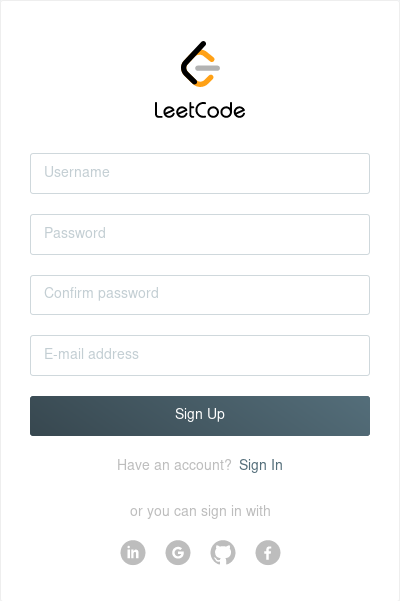
\includegraphics[width=\linewidth]{img/L2.png}
    \caption{Sign up page}
    \label{fig:L1}
\end{figure}

\section{Get started}
\section{Setting}
\section{System requirement}
\section{FAQ}
\section{terms and conditions}
\section{troubleshooting}


To begin with, you will need to create an account in order to acces the platform. It is possible to log in with you social network account such like facebook, google or github.

Once you have logged in, you can see this panel at the top.

click on your profile picture to acces your profile, you can see your personal progress. The interface is similaire to Github, you can track your activities (e.g: how many submission, succes rate etc).
I highly suggest you to not pay attention to the succes rate.

Let's start,
click on the <problem> panel, then you will see appear a list of questions, you can follow the problem order, or start with an random one, or reduce the selection to an specific domain.

Click an problem to start it, you will access to the "playground".
The playground is divided by 2 colums, at the left side, you can read the problem, most of them have few example to illutrate. Finally, at your right side, you have the coding environnement, one of the key feature of LeetCode is that you run it in an browser, there are nothing to install, you are totally free to use any* language to resolve the problem.
*LeetCode support most part of currently popular programming language (C++,Python2/3,C, Java, Javascript etc.)

Once your have done coding or you want to launch a test, all you have to do is click the "run code" at the right bottom, your code with be tested with the test-code next to you.
This process can be a little bit long, so most of time I'm used to run my code on my local machine with one specific test case.
At the end, if you are sure with solution, you can click the "submit" button, your code with be tested with all test-case. And finally if you pass all test-case, your solution is accepted and you can see the speed of your solution. Also, your program's performance is compared to the others, in my personal experience if you are under 20\% you can consider it as very fast, I do not advice you to target the 5\% since most of them are made of low level optimisation such like bitwise operation or syntaxique sugar for a specific programming language.
beetween 20 and 70\% I consider it as an good score, if you are over 70\%, that not too bad, you provided an succesful solution, there are probably some possible optimisation to perform.






test
\end{document}
